% Add image to the title page
\documentclass[aspectratio=169,10pt]{beamer}

\usepackage[utf8]{inputenc}
\usepackage{hyperref}
\hypersetup{
    colorlinks=true,
    pdftitle={TAC torchcvnn},
    pdfpagemode=FullScreen,
}

\def\tmp#1#2#3{%
  \definecolor{Hy#1color}{#2}{#3}%
  \hypersetup{#1color=Hy#1color}}
\tmp{link}{HTML}{800006}
\tmp{cite}{HTML}{2E7E2A}
\tmp{file}{HTML}{131877}
\tmp{url} {HTML}{8A0087}
\tmp{menu}{HTML}{727500}
\tmp{run} {HTML}{137776}

% Code syntax highlighter
\usepackage{minted}

\usepackage{tikz}
\usepackage{amssymb}
\usepackage{textpos}

\title{Ecosystem Project Proposal Summary}
\author{Jeremy Fix - torchcvnn}
\date{November 12th, 2024}
% \institute{The Institute that pays him}
% Add the image inside titlegraphics macro

% \setbeamersize{text margin left=15mm,text margin right=15mm, text margin top=10mm, text margin bottom=10mm}} 
\newcommand{\xmark}{%
\tikz[scale=0.23, color=red] {
    \draw[line width=0.7,line cap=round] (0,0) to [bend left=6] (1,1);
    \draw[line width=0.7,line cap=round] (0.2,0.95) to [bend right=3] (0.8,0.05);
}}

\newcommand{\cmark}{%
\tikz[scale=0.23, color=green] {
    \draw[line width=0.7,line cap=round] (0.25,0) to [bend left=10] (1,1);
    \draw[line width=0.8,line cap=round] (0,0.35) to [bend right=1] (0.23,0);
}}

\newcommand{\greencheck}{}%
\DeclareRobustCommand{\greencheck}{%
  \cmark
}
\newcommand{\redcross}{}%
\DeclareRobustCommand{\redcross}{%
  \xmark
}

\usepackage{newunicodechar}
\newcommand\warn{%
 \makebox[1.4em][c]{%
 \makebox[0pt][c]{\raisebox{.1em}{\small!}}%
 \makebox[0pt][c]{\color{red}\Large$\bigtriangleup$}}}%
\newunicodechar{⚠}{\warn}


\begin{document}


% \setbeamertemplate{headline}{\vskip10cm}

\definecolor{TitleColor}{rgb}{0.933,0.298,0.173}
\setbeamercolor{frametitle}{fg=TitleColor}
\setbeamerfont{frametitle}{size=\LARGE}
\setbeamerfont{block}{size=\LARGE,series=\bfseries}


\addtobeamertemplate{frametitle}{}{%
% \begin{textblock*}{100mm}(.85\textwidth,-1cm)

\includegraphics[height=0.5cm]{images/image2.png}
% \end{textblock*}
}
\setbeamertemplate{frametitle}{
	
\includegraphics[height=0.5cm]{images/image2.png}\\
    \vspace{-1cm}
	\begin{center}
    \insertframetitle
	\end{center}
}
% \setbeamertemplate{frametitle}[default][center]



{\usebackgroundtemplate{%
  
\includegraphics[width=\paperwidth,height=\paperheight]{images/bg.png}}
\begin{frame}

\titlepage
\end{frame}
}

\begin{frame}{Project Overview - Purpose and Mission}

% - Describe the purpose and mission of your project. What problem is it solving?
% - Why do you think this project is a good fit for the PyTorch Ecosystem?
% - How does this project augment the user experience, enable new capabilities, or speed up training/inference

\begin{block}{Purpose}
\vspace{4pt}
Several domains involve complex valued data, such as radar \cite{Barrachina2022}, MRI Fourier space \cite{Solomon2024,Hemidi2023}, optics \cite{Dinsdale2021}.\\

\vspace{4pt}

Pytorch already implements complex valued gradient descent (\href{https://pytorch.org/docs/stable/notes/autograd.html#autograd-for-complex-numbers}{Wirtinger Calculus}, see also \href{https://github.com/pytorch/pytorch/issues/33152}{\# 33152}) but lacks several complex valued capabilities such as :

\begin{itemize}
\item complex valued datasets (e.g. PolSF, ALOS2 or SLC loaders, fast-MRI, ...)
\item complex valued activation functions (Type A, Type B) % 
\item complex valued layers such as Dropout, BatchNorm, ...
\item complex valued initialization schemes, e.g. \cite{Trabelsi2018}
\end{itemize}

The objective is to provide robust, easy to use, complex valued neural networks + data loaders for PyTorch. 

\end{block}


% A Survey of Complex-Valued Neural Networks: https://arxiv.org/pdf/2101.12249

% Issue BatchNorm : https://github.com/pytorch/pytorch/issues/81749
% Activations : https://github.com/pytorch/pytorch/issues/47052
% Loss : https://github.com/pytorch/pytorch/issues/46642

\end{frame}

\begin{frame}{Project Overview - Purpose and Mission}

% Are there currently other Ecosystem or PyTorch projects similar to yours? If yes, what are they? How is your project different from them?


% ComplexPytorch : two large files , the operations does not have the same naming than pytorch.nn
%                hence would require refactoring
% cplmodule : same structure as pytorch 

\begin{block}{Other implementations with PyTorch}

\begin{itemize}
\item \href{https://github.com/wavefrontshaping/complexPyTorch}{complexPyTorch} by \cite{Matthes2021}, MIT license, 633 stars : \\
\greencheck several layers,  \redcross no CI/Tests, \redcross no docstrings, \redcross no type hints, \redcross no builtin datasets
\item \href{https://github.com/ivannz/cplxmodule}{cplxmodule}, by \cite{Nazarov2019}, 138 stars,\\
\greencheck several layers, \greencheck unit tests, \greencheck some documentation, \redcross no CI, \redcross using custom CplxParameter, \redcross no builtin datasets % needs to reimplement everything
\item \href{https://github.com/Roger-luo/pytorch-complex}{pytorch-complex}, archived since end 2019, 47 stars
\end{itemize}

\end{block}

\begin{block}{Other implementations with Tensorflow}

\begin{itemize}
\item \href{https://github.com/NEGU93/cvnn}{cvnn}, by \cite{Barrachina2022}, 164 stars
\item \href{https://github.com/JesperDramsch/keras-complex}{keras-complex} by \cite{Matthes2021}, 130 stars
\end{itemize}

\end{block}


\end{frame}


\begin{frame}{Project Summary}

% Please summarize the project details: repo URL, project Icon, Project License, GitHub
% handles of the project maintainers, number of stars, number of existing users, commit
% history (can just be the github insights chart)
%\vspace{-1cm}
\begin{itemize}
\item \href{https://github.com/jeremyfix/torchcvnn}{https://github.com/jeremyfix/torchcvnn}, \href{https://github.com/jeremyfix/torchcvnn/blob/main/LICENSE}{MIT License}, on \href{https://pypi.org/project/torchcvnn/}{pypi}
\item Documentation : \href{https://jeremyfix.github.io/torchcvnn/}{https://jeremyfix.github.io/torchcvnn/}
\item Maintainer : \href{https://github.com/jeremyfix}{@jeremyfix}
\item Number of stars : 7, Number of (known) users : 3
\item Dependencies : torch, numpy, pillow, requests
\item Torchscript or torch.compile : unused for now
\item \greencheck several layers, \greencheck Unit tests / Github actions, \greencheck mkdocs documentation, \greencheck docstrings and type hints, \greencheck builtin datasets

\begin{columns}[T] % align columns
\begin{column}{.3\textwidth}
\begin{center}
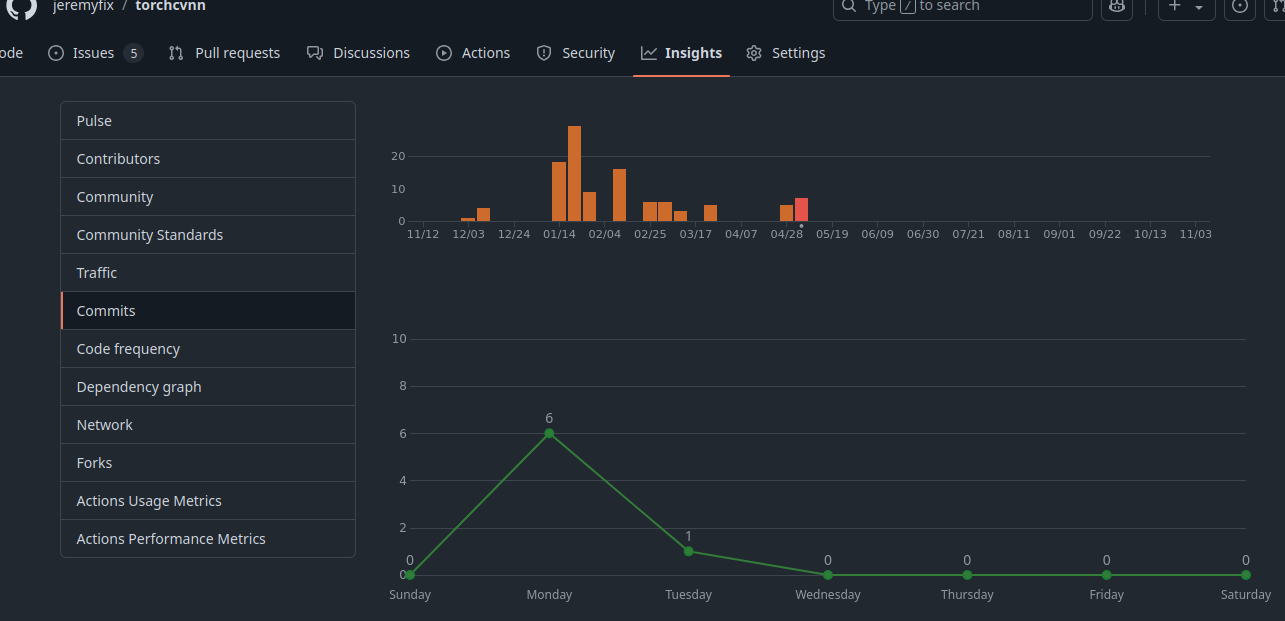
\includegraphics[width=\columnwidth]{images/commit_history.png}\\
Commit history
\end{center}
\end{column}%
\hfill%
\begin{column}{.3\textwidth}
\begin{center}
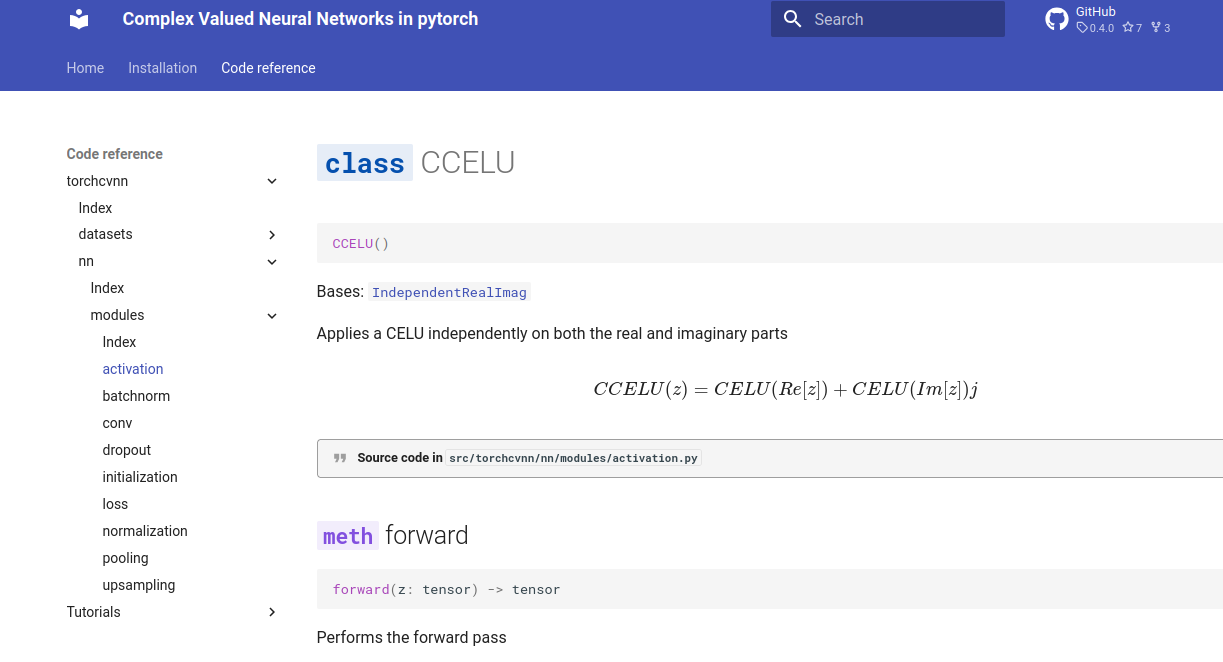
\includegraphics[width=\columnwidth]{images/documentation.png}\\
Mkdocs documentation
\end{center}
\end{column}%
\end{columns}

\end{itemize}

\end{frame}

% Use cases:
% - CineJENSE : NERF for reconstruction
% - Complex WGAN 

\begin{frame}[fragile]
\frametitle{Project Details}

\begin{block}{Architecture}
\begin{itemize}
\item mirrors torch package layout
\rule{\textwidth}{1pt}
\scriptsize
\begin{minted}{python}
    import torch.nn as n
    import torchcvnn.nn as c_nn
    
    def conv_block(in_c: int, out_c: int, cdtype: torch.dtype) -> List[nn.Module]:
        return [nn.Conv2d(in_c, out_c, kernel_size=3, stride=1, padding=1, dtype=cdtype),
            c_nn.BatchNorm2d(out_c),
            c_nn.Cardioid(),
            nn.Conv2d(out_c, out_c, kernel_size=3, stride=1, padding=1, dtype=cdtype),
            c_nn.BatchNorm2d(out_c),
            c_nn.Cardioid(),
            c_nn.AvgPool2d(kernel_size=2, stride=2, padding=0),
        ]
        cdtype = torch.complex64
        conv_model = nn.Sequential(
            *conv_block(1, 16, cdtype),
            *conv_block(16, 32, cdtype),
            nn.Flatten(),
        )
\end{minted}
\rule{\textwidth}{1pt}
\end{itemize}
\end{block}

\end{frame}


\begin{frame}[fragile]
\frametitle{Project Details}

\begin{block}{\href{https://jeremyfix.github.io/torchcvnn/reference/torchcvnn/datasets/}{Datasets} in torchcvnn/datasets/}

\begin{itemize}
    \item Generic \href{https://jeremyfix.github.io/torchcvnn/reference/torchcvnn/datasets/alos2/dataset/}{ALOS2} and \href{https://jeremyfix.github.io/torchcvnn/reference/torchcvnn/datasets/slc/dataset/}{SLC data loaders}
    \item PolSF or Bretigny SAR datasets
\begin{columns}[T] % align columns
\begin{column}{.6\textwidth}    
\rule{\textwidth}{1pt}
\scriptsize
\begin{minted}{python}
import torchcvnn
from torchcvnn.datasets.slc.dataset import SLCDataset

def get_pauli(data):
    # Returns Pauli in (H, W, C)
    HH = data["HH"]
    HV = data["HV"]
    VH = data["VH"]
    VV = data["VV"]
    return np.stack([HH-VV, HV+VH, HH+VV], axis=-1)
    
patch_size = (3000, 3000)
dataset = SLCDataset(
    rootdir,
    transform=get_pauli,
    patch_size=patch_size,
)
\end{minted}
\rule{\textwidth}{1pt}
\end{column}
\begin{column}{.3\textwidth}
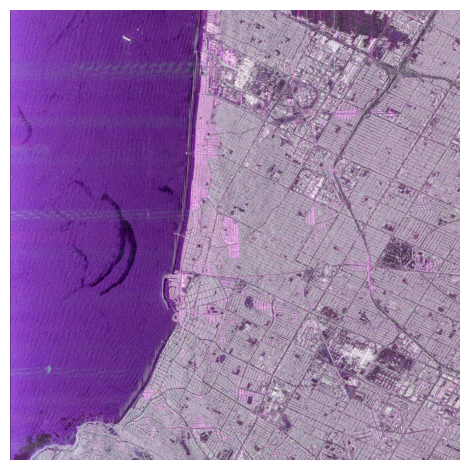
\includegraphics[width=\columnwidth]{images/slc_SSurge_15305.png}
\end{column}
\end{columns}
\end{itemize}

\end{block}

\end{frame}

\begin{frame}[fragile]
\frametitle{Project Details}

\begin{block}{\href{https://jeremyfix.github.io/torchcvnn/reference/torchcvnn/nn/modules/activation/}{Activations} in torchcvnn/nn/modules/activations.py}
\begin{itemize}
\item Type A using `IndependentRealImag` : CReLU, CPReLU, CELU, CCELU, CGELU, CSigmoid, CTanh
\rule{\textwidth}{1pt}
\scriptsize
\begin{minted}{python}
class IndependentRealImag(nn.Module):
    def __init__(self, fact: nn.Module):
        super().__init__()
        self.act_real = fact()
        self.act_imag = fact()
        
    def forward(self, z: torch.tensor) -> torch.tensor:
        return self.act_real(z.real) + self.act_imag(z.imag) * 1j
    
class CReLU(IndependentRealImag):
    def __init__(self) -> None:
        super().__init__(nn.ReLU)
\end{minted}
\rule{\textwidth}{1pt}
\normalsize
\item Type B : zReLU, zAbsReLU, zLeakyReLU, Mod, modReLU, Cardioid, 
\end{itemize}
\end{block}

\end{frame}



\begin{frame}[fragile]
\frametitle{Project Details}

\begin{block}{Layers in torchcvnn/nn/modules/*.py}
\begin{itemize}
    \item MaxPool2d (on mod), AvgPool2d, 
    \item BatchNorm1d, BatchNorm2d using a generic \href{https://github.com/jeremyfix/torchcvnn/blob/ede98e115649fcfc4f6098c6fefee758b4580449/src/torchcvnn/nn/modules/batchnorm.py#L151}{BatchNormNd} for tensors of shape \begin{verbatim}(batch_size, features, d1, d2, ..)\end{verbatim} with $features$ means and covariances
    \item LayerNorm 
    \item ConvTranspose2d, Upsample (nn.Upsample on real/imag)
    \item Dropout, Dropout2d
\rule{\textwidth}{1pt}
\scriptsize
\begin{minted}{python}
    def forward(self, z: torch.Tensor) -> torch.Tensor:
        mask = torch.nn.functional.dropout(
            torch.ones(z.shape), self.p, training=self.training
        ).to(z.device)
        return mask * z
\end{minted}
\rule{\textwidth}{1pt}
\normalsize    
\end{itemize}


\end{block}

\end{frame}

\begin{frame}[fragile]
\frametitle{Project Details}

\begin{block}{Unit tests}

\begin{itemize}
\item Ran within github actions using pytest, see \href{https://github.com/jeremyfix/torchcvnn/blob/main/.github/workflows/test.yml}{test.yml}
\item several "call tests", some unit tests, e.g. BatchNorm
\end{itemize}
\scriptsize
\begin{minted}{python}
def test_batchnorm1d():
    B, C = 20, 16
    m = c_nn.BatchNorm1d(C)

    x = torch.randn((B, C), dtype=torch.complex64)
    output = m(x)

    # Compute the variance/covariance
    xc = output.transpose(0, 1).reshape(C, -1)  # C, B
    mus = xc.mean(axis=-1)  # 16 means
    xc_real = torch.view_as_real(xc)
    covs = bn.batch_cov(xc_real)  # 16 covariances matrices

    # All the mus must be 0's
    # For some reasons, this is not exactly 0
    assert torch.allclose(mus, torch.zeros_like(mus), atol=1e-7)
    # All the covs must be identities
    id_cov = 0.5 * torch.eye(2).tile(C, 1, 1)
    assert torch.allclose(covs, id_cov, atol=1e-7)
\end{minted}
\normalsize 


\end{block}

\end{frame}



\begin{frame}{Project Roadmap}

\begin{block}{Planned enhancements}
\begin{itemize}
\item provide more builtin datasets wrappers : fastMRI (\href{https://github.com/jeremyfix/torchcvnn/issues/20}{issue #20}), MSTAR (\href{https://github.com/jeremyfix/torchcvnn/issues/18}{issue #18})
\item implement standard models, e.g. transformers (⚠ attention layer using Softmax requires a specific implementation)
\end{itemize}
\end{block}

\begin{block}{Current projects involving torchcvnn, bringing support}

\begin{itemize}
\item Quentin Gabot, PhD Thesis on generative AI for SAR imagery, started 2023
\item Xan-Huy Ngugyen, PhD Thesis on self-supervized learning, started 2024
\item CentraleSupelec Master student project on self-supervized CVNNs, extending MERLIN-seg\cite{Dalasso2024}and SAFE \cite{Muzeau2024}
\end{itemize}

\end{block}

\end{frame}

\section{Request to TAC}
\begin{frame}{Request to TAC}

\begin{block}{Proposal}

That torchcvnn is adopted as a project of the PyTorch Foundation Ecosystem Tools.
\end{block}

\end{frame}


\section{Use cases}

\begin{frame}{Use cases}

\begin{itemize}
\item Complex valued NERF for cardiac reconstruction, based on \cite{Hemidi2023}
\item Complex valued WGAN \cite{Dhedin2024}
\item Complex valued auto-encoders for SAR \cite{Gabot2024}
\end{itemize}

\end{frame}

\section{References}

\bibliographystyle{apalike}
\bibliography{biblio}

\end{document}
